%	
%\renewcommand{\theequation}{\theenumi}
%\begin{enumerate}[label=\arabic*.,ref=\thesubsection.\theenumi]
%\numberwithin{equation}{enumi}

\item Balance the following chemical equation.
%
\begin{align}
\label{eq:chem_balance}
Fe+H_2O &\rightarrow Fe_3O_4 + H_2
\end{align}
%
\solution Let the balanced version of \eqref{eq:chem_balance} be 
%
\begin{align}
\label{eq:chem_balance_unsol}
x_1Fe+x_2H_2 O &\rightarrow x_3Fe_3 O_4 + x_4H_2
\end{align}
%
which results in the following equations
%
\begin{align}
\begin{split}
\brak{x_1 -3x_3}Fe &= 0
\\
\brak{2x_2 -2x_4}H &= 0
\\
\brak{x_2 -4x_3}O &= 0
\end{split}
\end{align}
which can be expressed as
\begin{align}
\begin{split}
x_1 + 0.x_2 -3x_3 +0.x_4&= 0
\\
0.x_1+2x_2 +0.x_3-2x_4 &= 0
\\
0.x_1+x_2 -4x_3+ 0.x_4 &= 0
\end{split}
\end{align}
%
resulting in the matrix equation
\begin{align}
\label{eq:chem_balance_mat_eq}
\begin{split}
\myvec{
1 & 0 & -3 & 0
\\
0 & 2 & 0 & -2
\\
0 & 1 & -4 & 0
}
\vec{x} &= \vec{0}
\end{split}
\end{align}
%
where
\begin{align}
\vec{x} = \myvec{x_1 \\ x_2 \\ x_3 \\ x_4} 
\end{align}
%\item Solve \eqref{eq:chem_balance_unsol} by row reducing 
%the matrix in \eqref{eq:chem_balance_mat_eq}.
%\\
%\solution  
\eqref{eq:chem_balance_mat_eq} can be row reduced as follows
%
\begin{align}
\label{eq:chem_balance_mat_row}
\myvec{
1 & 0 & -3 & 0
\\
0 & 2 & 0 & -2
\\
0 & 1 & -4 & 0
}
 \xleftrightarrow[]{R_2 \leftarrow \frac{R_2}{2}}
\myvec{
1 & 0 & -3 & 0
\\
0 & 1 & 0 & -1
\\
0 & 1 & -4 & 0
}
\\
 \xleftrightarrow[]{R_3\leftarrow R_3-R_2}
\myvec{
1 & 0 & -3 & 0
\\
0 & 1 & 0 & -1
\\
0 & 0 & -4 & 1
}
\\
 \xleftrightarrow[]{R_1\leftarrow 4R_1-3R_3}
\myvec{
4 & 0 & 0 & -3
\\
0 & 1 & 0 & -1
\\
0 & 0 & -4 & 1
}
\\
 \xleftrightarrow[R_3 \leftarrow -\frac{1}{4}R_3]{R_1\leftarrow \frac{1}{4}}
\myvec{
1 & 0 & 0 & -\frac{3}{4}
\\
0 & 1 & 0 & -1
\\
0 & 0 & 1 & -\frac{1}{4}
}
\end{align}
%
Thus, 
\begin{align}
\label{eq:chem_balance_mat_sol}
x_1 &= \frac{3}{4}x_4, x_2 = x_4, x_3 = \frac{1}{4}x_4
\\
\\
\implies 
\vec{x} &= x_4\myvec{\frac{3}{4} \\ 1 \\ \frac{1}{4} \\ 1}= \myvec{3 \\ 4 \\ 1 \\ 4}
\end{align}
%
upon substituting $x_4 = 4$.
%
\eqref{eq:chem_balance_unsol} then becomes
%
\begin{align}
\label{eq:chem_balance_final}
3Fe+4H_2 O &\rightarrow Fe_3 O_4 + 4H_2
\end{align}

\item Consider the following information regarding the number of men and women workers in the three factories I,II and III

\begin{tabular}{ |c|c|c| } 
\hline
 & Men Workers & Women Workers \\
\hline
\multirow{3}{4em}{I \\II \\III} & 30 & 25\\ 
& 25 & 31 \\ 
&27 & 26 \\ 
\hline
\end{tabular}\\
Represent the above information in the form of a 3 $\times$ 2 matrix. What does the entry
in the third row and second column represent?\\


 \item  If a matrix has 8 elements, what are the possible orders it can have?\\
    \item Construct a 3 $\times$ 2 matrix whose elements are given by $a_{ij}=\frac{1}{2}\abs{i-3j}$\\
    \item \myvec{x+3 &z+4 &2y-7\\-6 &a-1 &0\\b-3 &-21 &0}=\myvec{0 &6 &3y-2\\-6 &-3 &2c+2\\2b+4 &-21 &0}\\
    Find the values of a,b,c,x,y and z.\\
\solution 
\input{./solutions/5/chapters/lines/docq7.tex}
    \item Find the values of a,b,c and d from the following equation:\\
    \myvec{2a+b &a-2b\\5c-d &4c+3d}=\myvec{4 &-3\\11 &24}\\
\solution 
%
\begin{align}
    E(X) &= \frac{1}{\sqrt{2\pi}} \int_{-\infty}^{\infty} x e^{-\frac{x^2}{2}}dx\\
    &=0 \quad \brak{ \text{ odd function}}
\end{align}
\begin{align}
    E\brak{X^2}&= \frac{1}{\sqrt{2\pi}}\int_{-\infty}^{\infty} x^2
e^ {-\frac{x^2}{2}} dx \quad \brak{even function}\\
    &= \frac{2}{\sqrt{2\pi}} \int_{0}^{\infty} x^2 e^{-\frac{x^2}{2}} dx\\
    &= \frac{2}{\sqrt{2\pi}}\int_{0}^{\infty}\sqrt{2u}e^{-u} du \quad\brak{Let \frac{x^2}{2}= u}\\
    &= \frac{2}{\sqrt{\pi}} \int_{0}^{\infty} e^{-u} u^{\frac{3}{2}-1} du\\
    &= \frac{2}{\sqrt{\pi}} \Gamma\brak{{\frac{3}{2}}}\\
    &= \frac{1}{\sqrt{\pi}}\Gamma\brak{\frac{1}{2}} \\
    &= 1
\end{align}
where we have used the fact that
\begin{align}
\quad\because \Gamma(n)= (n-1)\Gamma(n-1); \Gamma\brak{\frac{1}{2}}=\sqrt{\pi}
\end{align}
%
Thus, the  variance is
\begin{align}
    \sigma^2 =  E\brak X^2 - E^2\brak X = 1
\end{align}

    \item Given A=\myvec{\sqrt{3} &1 &-1\\2 &3 &0} and B=\myvec{2 &\sqrt{5} &1\\-2 &3 &\frac{1}{2}}, find A+B.\\\solution 
%
\begin{align}
    E(X) &= \frac{1}{\sqrt{2\pi}} \int_{-\infty}^{\infty} x e^{-\frac{x^2}{2}}dx\\
    &=0 \quad \brak{ \text{ odd function}}
\end{align}
\begin{align}
    E\brak{X^2}&= \frac{1}{\sqrt{2\pi}}\int_{-\infty}^{\infty} x^2
e^ {-\frac{x^2}{2}} dx \quad \brak{even function}\\
    &= \frac{2}{\sqrt{2\pi}} \int_{0}^{\infty} x^2 e^{-\frac{x^2}{2}} dx\\
    &= \frac{2}{\sqrt{2\pi}}\int_{0}^{\infty}\sqrt{2u}e^{-u} du \quad\brak{Let \frac{x^2}{2}= u}\\
    &= \frac{2}{\sqrt{\pi}} \int_{0}^{\infty} e^{-u} u^{\frac{3}{2}-1} du\\
    &= \frac{2}{\sqrt{\pi}} \Gamma\brak{{\frac{3}{2}}}\\
    &= \frac{1}{\sqrt{\pi}}\Gamma\brak{\frac{1}{2}} \\
    &= 1
\end{align}
where we have used the fact that
\begin{align}
\quad\because \Gamma(n)= (n-1)\Gamma(n-1); \Gamma\brak{\frac{1}{2}}=\sqrt{\pi}
\end{align}
%
Thus, the  variance is
\begin{align}
    \sigma^2 =  E\brak X^2 - E^2\brak X = 1
\end{align}

\item In the matrix A=\myvec{2 &5 &19 &-7\\ 35 &-2 &\frac{5}{2} &12 \\ \sqrt{3} &1 &-5 &17}, write
\begin{enumerate}
\item The order of the matrix
\item The number of elements
\item Write the elements $a_{31},a_{21},a_{33},a_{24},a_{23}.$
\end{enumerate}
\solution 
%
\begin{align}
    E(X) &= \frac{1}{\sqrt{2\pi}} \int_{-\infty}^{\infty} x e^{-\frac{x^2}{2}}dx\\
    &=0 \quad \brak{ \text{ odd function}}
\end{align}
\begin{align}
    E\brak{X^2}&= \frac{1}{\sqrt{2\pi}}\int_{-\infty}^{\infty} x^2
e^ {-\frac{x^2}{2}} dx \quad \brak{even function}\\
    &= \frac{2}{\sqrt{2\pi}} \int_{0}^{\infty} x^2 e^{-\frac{x^2}{2}} dx\\
    &= \frac{2}{\sqrt{2\pi}}\int_{0}^{\infty}\sqrt{2u}e^{-u} du \quad\brak{Let \frac{x^2}{2}= u}\\
    &= \frac{2}{\sqrt{\pi}} \int_{0}^{\infty} e^{-u} u^{\frac{3}{2}-1} du\\
    &= \frac{2}{\sqrt{\pi}} \Gamma\brak{{\frac{3}{2}}}\\
    &= \frac{1}{\sqrt{\pi}}\Gamma\brak{\frac{1}{2}} \\
    &= 1
\end{align}
where we have used the fact that
\begin{align}
\quad\because \Gamma(n)= (n-1)\Gamma(n-1); \Gamma\brak{\frac{1}{2}}=\sqrt{\pi}
\end{align}
%
Thus, the  variance is
\begin{align}
    \sigma^2 =  E\brak X^2 - E^2\brak X = 1
\end{align}


\item If a matrix has 24 elements,what are the possible orders it can have? What,if it has 13 elements?\\
\solution 
%
\begin{align}
    E(X) &= \frac{1}{\sqrt{2\pi}} \int_{-\infty}^{\infty} x e^{-\frac{x^2}{2}}dx\\
    &=0 \quad \brak{ \text{ odd function}}
\end{align}
\begin{align}
    E\brak{X^2}&= \frac{1}{\sqrt{2\pi}}\int_{-\infty}^{\infty} x^2
e^ {-\frac{x^2}{2}} dx \quad \brak{even function}\\
    &= \frac{2}{\sqrt{2\pi}} \int_{0}^{\infty} x^2 e^{-\frac{x^2}{2}} dx\\
    &= \frac{2}{\sqrt{2\pi}}\int_{0}^{\infty}\sqrt{2u}e^{-u} du \quad\brak{Let \frac{x^2}{2}= u}\\
    &= \frac{2}{\sqrt{\pi}} \int_{0}^{\infty} e^{-u} u^{\frac{3}{2}-1} du\\
    &= \frac{2}{\sqrt{\pi}} \Gamma\brak{{\frac{3}{2}}}\\
    &= \frac{1}{\sqrt{\pi}}\Gamma\brak{\frac{1}{2}} \\
    &= 1
\end{align}
where we have used the fact that
\begin{align}
\quad\because \Gamma(n)= (n-1)\Gamma(n-1); \Gamma\brak{\frac{1}{2}}=\sqrt{\pi}
\end{align}
%
Thus, the  variance is
\begin{align}
    \sigma^2 =  E\brak X^2 - E^2\brak X = 1
\end{align}

\item If a matrix has 18 elements,what are the possible orders it can have? What,if it has 5 elements?\\
\\
\solution 
%
\begin{align}
    E(X) &= \frac{1}{\sqrt{2\pi}} \int_{-\infty}^{\infty} x e^{-\frac{x^2}{2}}dx\\
    &=0 \quad \brak{ \text{ odd function}}
\end{align}
\begin{align}
    E\brak{X^2}&= \frac{1}{\sqrt{2\pi}}\int_{-\infty}^{\infty} x^2
e^ {-\frac{x^2}{2}} dx \quad \brak{even function}\\
    &= \frac{2}{\sqrt{2\pi}} \int_{0}^{\infty} x^2 e^{-\frac{x^2}{2}} dx\\
    &= \frac{2}{\sqrt{2\pi}}\int_{0}^{\infty}\sqrt{2u}e^{-u} du \quad\brak{Let \frac{x^2}{2}= u}\\
    &= \frac{2}{\sqrt{\pi}} \int_{0}^{\infty} e^{-u} u^{\frac{3}{2}-1} du\\
    &= \frac{2}{\sqrt{\pi}} \Gamma\brak{{\frac{3}{2}}}\\
    &= \frac{1}{\sqrt{\pi}}\Gamma\brak{\frac{1}{2}} \\
    &= 1
\end{align}
where we have used the fact that
\begin{align}
\quad\because \Gamma(n)= (n-1)\Gamma(n-1); \Gamma\brak{\frac{1}{2}}=\sqrt{\pi}
\end{align}
%
Thus, the  variance is
\begin{align}
    \sigma^2 =  E\brak X^2 - E^2\brak X = 1
\end{align}

%
\item Construct a $2 \times 2$ matrix,A=[$a_{ij}$],whose elements are given by:\\
(i) $a_{ij}$=$\frac{(i+j)^2}{2}$\ (ii) $a_{ij}$=$\frac{i}{j}$\ (iii) $a_{ij}$=$\frac{(i+2j)^2}{2}$\\
\solution 
%
\begin{align}
    E(X) &= \frac{1}{\sqrt{2\pi}} \int_{-\infty}^{\infty} x e^{-\frac{x^2}{2}}dx\\
    &=0 \quad \brak{ \text{ odd function}}
\end{align}
\begin{align}
    E\brak{X^2}&= \frac{1}{\sqrt{2\pi}}\int_{-\infty}^{\infty} x^2
e^ {-\frac{x^2}{2}} dx \quad \brak{even function}\\
    &= \frac{2}{\sqrt{2\pi}} \int_{0}^{\infty} x^2 e^{-\frac{x^2}{2}} dx\\
    &= \frac{2}{\sqrt{2\pi}}\int_{0}^{\infty}\sqrt{2u}e^{-u} du \quad\brak{Let \frac{x^2}{2}= u}\\
    &= \frac{2}{\sqrt{\pi}} \int_{0}^{\infty} e^{-u} u^{\frac{3}{2}-1} du\\
    &= \frac{2}{\sqrt{\pi}} \Gamma\brak{{\frac{3}{2}}}\\
    &= \frac{1}{\sqrt{\pi}}\Gamma\brak{\frac{1}{2}} \\
    &= 1
\end{align}
where we have used the fact that
\begin{align}
\quad\because \Gamma(n)= (n-1)\Gamma(n-1); \Gamma\brak{\frac{1}{2}}=\sqrt{\pi}
\end{align}
%
Thus, the  variance is
\begin{align}
    \sigma^2 =  E\brak X^2 - E^2\brak X = 1
\end{align}

\item Construct a $3\times 4$ matrix,whose elements are given by:\\
(i) $a_{ij}$=$\frac{1}{2}\abs{-3i+j}$ (ii) $a_{ij}$=2i-j\\
\solution 
\input{./solutions/5/chapters/lines/docq13.tex}
\item Find the values of x,y and z from the following equations:\\
(i) \myvec{4 &3\\x &5} = \myvec{y &z\\1 &5} (ii) \myvec{x+y &2\\5+z &xy} = \myvec{6 &2\\5 &8} (iii) \myvec{x+y+z\\x+y\\y+z}=\myvec{9\\5\\7}\\
\\
\solution 
%
\begin{align}
    E(X) &= \frac{1}{\sqrt{2\pi}} \int_{-\infty}^{\infty} x e^{-\frac{x^2}{2}}dx\\
    &=0 \quad \brak{ \text{ odd function}}
\end{align}
\begin{align}
    E\brak{X^2}&= \frac{1}{\sqrt{2\pi}}\int_{-\infty}^{\infty} x^2
e^ {-\frac{x^2}{2}} dx \quad \brak{even function}\\
    &= \frac{2}{\sqrt{2\pi}} \int_{0}^{\infty} x^2 e^{-\frac{x^2}{2}} dx\\
    &= \frac{2}{\sqrt{2\pi}}\int_{0}^{\infty}\sqrt{2u}e^{-u} du \quad\brak{Let \frac{x^2}{2}= u}\\
    &= \frac{2}{\sqrt{\pi}} \int_{0}^{\infty} e^{-u} u^{\frac{3}{2}-1} du\\
    &= \frac{2}{\sqrt{\pi}} \Gamma\brak{{\frac{3}{2}}}\\
    &= \frac{1}{\sqrt{\pi}}\Gamma\brak{\frac{1}{2}} \\
    &= 1
\end{align}
where we have used the fact that
\begin{align}
\quad\because \Gamma(n)= (n-1)\Gamma(n-1); \Gamma\brak{\frac{1}{2}}=\sqrt{\pi}
\end{align}
%
Thus, the  variance is
\begin{align}
    \sigma^2 =  E\brak X^2 - E^2\brak X = 1
\end{align}

\item Compute the indicated products.
\begin{enumerate}
\item \myvec{a &b\\-b &a}\myvec{a &-b\\b &a} \\
\solution 
%
\begin{align}
    E(X) &= \frac{1}{\sqrt{2\pi}} \int_{-\infty}^{\infty} x e^{-\frac{x^2}{2}}dx\\
    &=0 \quad \brak{ \text{ odd function}}
\end{align}
\begin{align}
    E\brak{X^2}&= \frac{1}{\sqrt{2\pi}}\int_{-\infty}^{\infty} x^2
e^ {-\frac{x^2}{2}} dx \quad \brak{even function}\\
    &= \frac{2}{\sqrt{2\pi}} \int_{0}^{\infty} x^2 e^{-\frac{x^2}{2}} dx\\
    &= \frac{2}{\sqrt{2\pi}}\int_{0}^{\infty}\sqrt{2u}e^{-u} du \quad\brak{Let \frac{x^2}{2}= u}\\
    &= \frac{2}{\sqrt{\pi}} \int_{0}^{\infty} e^{-u} u^{\frac{3}{2}-1} du\\
    &= \frac{2}{\sqrt{\pi}} \Gamma\brak{{\frac{3}{2}}}\\
    &= \frac{1}{\sqrt{\pi}}\Gamma\brak{\frac{1}{2}} \\
    &= 1
\end{align}
where we have used the fact that
\begin{align}
\quad\because \Gamma(n)= (n-1)\Gamma(n-1); \Gamma\brak{\frac{1}{2}}=\sqrt{\pi}
\end{align}
%
Thus, the  variance is
\begin{align}
    \sigma^2 =  E\brak X^2 - E^2\brak X = 1
\end{align}

\item \myvec{1\\2\\3}\myvec{2 &3 &4} 
\\
\solution 
%
\begin{align}
    E(X) &= \frac{1}{\sqrt{2\pi}} \int_{-\infty}^{\infty} x e^{-\frac{x^2}{2}}dx\\
    &=0 \quad \brak{ \text{ odd function}}
\end{align}
\begin{align}
    E\brak{X^2}&= \frac{1}{\sqrt{2\pi}}\int_{-\infty}^{\infty} x^2
e^ {-\frac{x^2}{2}} dx \quad \brak{even function}\\
    &= \frac{2}{\sqrt{2\pi}} \int_{0}^{\infty} x^2 e^{-\frac{x^2}{2}} dx\\
    &= \frac{2}{\sqrt{2\pi}}\int_{0}^{\infty}\sqrt{2u}e^{-u} du \quad\brak{Let \frac{x^2}{2}= u}\\
    &= \frac{2}{\sqrt{\pi}} \int_{0}^{\infty} e^{-u} u^{\frac{3}{2}-1} du\\
    &= \frac{2}{\sqrt{\pi}} \Gamma\brak{{\frac{3}{2}}}\\
    &= \frac{1}{\sqrt{\pi}}\Gamma\brak{\frac{1}{2}} \\
    &= 1
\end{align}
where we have used the fact that
\begin{align}
\quad\because \Gamma(n)= (n-1)\Gamma(n-1); \Gamma\brak{\frac{1}{2}}=\sqrt{\pi}
\end{align}
%
Thus, the  variance is
\begin{align}
    \sigma^2 =  E\brak X^2 - E^2\brak X = 1
\end{align}

\item \myvec{1 &-2\\2 &3}\myvec{1 &2 &3\\2 &3 &1} \\
\end{enumerate}
\item Simplify $\cos\theta$$\myvec{\cos\theta &\sin\theta\\ -\sin\theta &\cos\theta}$+$\sin\theta$$\myvec{\sin\theta &-\cos\theta\\ \cos\theta &\sin\theta}$\\
\solution 
%
\begin{align}
    E(X) &= \frac{1}{\sqrt{2\pi}} \int_{-\infty}^{\infty} x e^{-\frac{x^2}{2}}dx\\
    &=0 \quad \brak{ \text{ odd function}}
\end{align}
\begin{align}
    E\brak{X^2}&= \frac{1}{\sqrt{2\pi}}\int_{-\infty}^{\infty} x^2
e^ {-\frac{x^2}{2}} dx \quad \brak{even function}\\
    &= \frac{2}{\sqrt{2\pi}} \int_{0}^{\infty} x^2 e^{-\frac{x^2}{2}} dx\\
    &= \frac{2}{\sqrt{2\pi}}\int_{0}^{\infty}\sqrt{2u}e^{-u} du \quad\brak{Let \frac{x^2}{2}= u}\\
    &= \frac{2}{\sqrt{\pi}} \int_{0}^{\infty} e^{-u} u^{\frac{3}{2}-1} du\\
    &= \frac{2}{\sqrt{\pi}} \Gamma\brak{{\frac{3}{2}}}\\
    &= \frac{1}{\sqrt{\pi}}\Gamma\brak{\frac{1}{2}} \\
    &= 1
\end{align}
where we have used the fact that
\begin{align}
\quad\because \Gamma(n)= (n-1)\Gamma(n-1); \Gamma\brak{\frac{1}{2}}=\sqrt{\pi}
\end{align}
%
Thus, the  variance is
\begin{align}
    \sigma^2 =  E\brak X^2 - E^2\brak X = 1
\end{align}

\item Find X and Y,if\\
(i)X+Y=\myvec{7 &0\\2 &5} and X-Y=\myvec{3 &0\\0 &3}\\
(ii)2X+3Y=\myvec{2 &3\\4 &0} and 3X+2Y=\myvec{2 &-2\\-1 &5}\\ 
\solution 
%
\begin{align}
    E(X) &= \frac{1}{\sqrt{2\pi}} \int_{-\infty}^{\infty} x e^{-\frac{x^2}{2}}dx\\
    &=0 \quad \brak{ \text{ odd function}}
\end{align}
\begin{align}
    E\brak{X^2}&= \frac{1}{\sqrt{2\pi}}\int_{-\infty}^{\infty} x^2
e^ {-\frac{x^2}{2}} dx \quad \brak{even function}\\
    &= \frac{2}{\sqrt{2\pi}} \int_{0}^{\infty} x^2 e^{-\frac{x^2}{2}} dx\\
    &= \frac{2}{\sqrt{2\pi}}\int_{0}^{\infty}\sqrt{2u}e^{-u} du \quad\brak{Let \frac{x^2}{2}= u}\\
    &= \frac{2}{\sqrt{\pi}} \int_{0}^{\infty} e^{-u} u^{\frac{3}{2}-1} du\\
    &= \frac{2}{\sqrt{\pi}} \Gamma\brak{{\frac{3}{2}}}\\
    &= \frac{1}{\sqrt{\pi}}\Gamma\brak{\frac{1}{2}} \\
    &= 1
\end{align}
where we have used the fact that
\begin{align}
\quad\because \Gamma(n)= (n-1)\Gamma(n-1); \Gamma\brak{\frac{1}{2}}=\sqrt{\pi}
\end{align}
%
Thus, the  variance is
\begin{align}
    \sigma^2 =  E\brak X^2 - E^2\brak X = 1
\end{align}

\item Find X if Y=\myvec{3 &2\\1 &4} and 2X+Y=\myvec{1 &0\\-3 &2}\\
\solution 
%
\begin{align}
    E(X) &= \frac{1}{\sqrt{2\pi}} \int_{-\infty}^{\infty} x e^{-\frac{x^2}{2}}dx\\
    &=0 \quad \brak{ \text{ odd function}}
\end{align}
\begin{align}
    E\brak{X^2}&= \frac{1}{\sqrt{2\pi}}\int_{-\infty}^{\infty} x^2
e^ {-\frac{x^2}{2}} dx \quad \brak{even function}\\
    &= \frac{2}{\sqrt{2\pi}} \int_{0}^{\infty} x^2 e^{-\frac{x^2}{2}} dx\\
    &= \frac{2}{\sqrt{2\pi}}\int_{0}^{\infty}\sqrt{2u}e^{-u} du \quad\brak{Let \frac{x^2}{2}= u}\\
    &= \frac{2}{\sqrt{\pi}} \int_{0}^{\infty} e^{-u} u^{\frac{3}{2}-1} du\\
    &= \frac{2}{\sqrt{\pi}} \Gamma\brak{{\frac{3}{2}}}\\
    &= \frac{1}{\sqrt{\pi}}\Gamma\brak{\frac{1}{2}} \\
    &= 1
\end{align}
where we have used the fact that
\begin{align}
\quad\because \Gamma(n)= (n-1)\Gamma(n-1); \Gamma\brak{\frac{1}{2}}=\sqrt{\pi}
\end{align}
%
Thus, the  variance is
\begin{align}
    \sigma^2 =  E\brak X^2 - E^2\brak X = 1
\end{align}

\item If F(x)=$\myvec{\cos x &-\sin x &0\\ \sin x &\cos x &0\\0 &0 &1}$\\,show that F(x)F(y)=F(x+y)\\
\solution 
%
\begin{align}
    E(X) &= \frac{1}{\sqrt{2\pi}} \int_{-\infty}^{\infty} x e^{-\frac{x^2}{2}}dx\\
    &=0 \quad \brak{ \text{ odd function}}
\end{align}
\begin{align}
    E\brak{X^2}&= \frac{1}{\sqrt{2\pi}}\int_{-\infty}^{\infty} x^2
e^ {-\frac{x^2}{2}} dx \quad \brak{even function}\\
    &= \frac{2}{\sqrt{2\pi}} \int_{0}^{\infty} x^2 e^{-\frac{x^2}{2}} dx\\
    &= \frac{2}{\sqrt{2\pi}}\int_{0}^{\infty}\sqrt{2u}e^{-u} du \quad\brak{Let \frac{x^2}{2}= u}\\
    &= \frac{2}{\sqrt{\pi}} \int_{0}^{\infty} e^{-u} u^{\frac{3}{2}-1} du\\
    &= \frac{2}{\sqrt{\pi}} \Gamma\brak{{\frac{3}{2}}}\\
    &= \frac{1}{\sqrt{\pi}}\Gamma\brak{\frac{1}{2}} \\
    &= 1
\end{align}
where we have used the fact that
\begin{align}
\quad\because \Gamma(n)= (n-1)\Gamma(n-1); \Gamma\brak{\frac{1}{2}}=\sqrt{\pi}
\end{align}
%
Thus, the  variance is
\begin{align}
    \sigma^2 =  E\brak X^2 - E^2\brak X = 1
\end{align}

\item Find $A^{2}-5A+6I$,if A = \myvec{2 &0 &1\\2 &1 &3\\1 &-1 &0}\\
\solution 
%
\begin{align}
    E(X) &= \frac{1}{\sqrt{2\pi}} \int_{-\infty}^{\infty} x e^{-\frac{x^2}{2}}dx\\
    &=0 \quad \brak{ \text{ odd function}}
\end{align}
\begin{align}
    E\brak{X^2}&= \frac{1}{\sqrt{2\pi}}\int_{-\infty}^{\infty} x^2
e^ {-\frac{x^2}{2}} dx \quad \brak{even function}\\
    &= \frac{2}{\sqrt{2\pi}} \int_{0}^{\infty} x^2 e^{-\frac{x^2}{2}} dx\\
    &= \frac{2}{\sqrt{2\pi}}\int_{0}^{\infty}\sqrt{2u}e^{-u} du \quad\brak{Let \frac{x^2}{2}= u}\\
    &= \frac{2}{\sqrt{\pi}} \int_{0}^{\infty} e^{-u} u^{\frac{3}{2}-1} du\\
    &= \frac{2}{\sqrt{\pi}} \Gamma\brak{{\frac{3}{2}}}\\
    &= \frac{1}{\sqrt{\pi}}\Gamma\brak{\frac{1}{2}} \\
    &= 1
\end{align}
where we have used the fact that
\begin{align}
\quad\because \Gamma(n)= (n-1)\Gamma(n-1); \Gamma\brak{\frac{1}{2}}=\sqrt{\pi}
\end{align}
%
Thus, the  variance is
\begin{align}
    \sigma^2 =  E\brak X^2 - E^2\brak X = 1
\end{align}

\item If A=\myvec{1 &0 &2\\0 &2 &1\\2 &0 &3},prove that $A^3-6A^2+7A+2I=0$\\
\solution 
%
\begin{align}
    E(X) &= \frac{1}{\sqrt{2\pi}} \int_{-\infty}^{\infty} x e^{-\frac{x^2}{2}}dx\\
    &=0 \quad \brak{ \text{ odd function}}
\end{align}
\begin{align}
    E\brak{X^2}&= \frac{1}{\sqrt{2\pi}}\int_{-\infty}^{\infty} x^2
e^ {-\frac{x^2}{2}} dx \quad \brak{even function}\\
    &= \frac{2}{\sqrt{2\pi}} \int_{0}^{\infty} x^2 e^{-\frac{x^2}{2}} dx\\
    &= \frac{2}{\sqrt{2\pi}}\int_{0}^{\infty}\sqrt{2u}e^{-u} du \quad\brak{Let \frac{x^2}{2}= u}\\
    &= \frac{2}{\sqrt{\pi}} \int_{0}^{\infty} e^{-u} u^{\frac{3}{2}-1} du\\
    &= \frac{2}{\sqrt{\pi}} \Gamma\brak{{\frac{3}{2}}}\\
    &= \frac{1}{\sqrt{\pi}}\Gamma\brak{\frac{1}{2}} \\
    &= 1
\end{align}
where we have used the fact that
\begin{align}
\quad\because \Gamma(n)= (n-1)\Gamma(n-1); \Gamma\brak{\frac{1}{2}}=\sqrt{\pi}
\end{align}
%
Thus, the  variance is
\begin{align}
    \sigma^2 =  E\brak X^2 - E^2\brak X = 1
\end{align}

\item If A=$\myvec{0 &-\tan\frac{\alpha}{2}\\  \tan\frac{\alpha}{2} &0}$ and I is the identity matrix of order 2,show that \\I+A=(I-A)$\myvec{\cos\alpha &-\sin\alpha\\\sin\alpha &\cos\alpha}$\\
\solution 
%
\begin{align}
    E(X) &= \frac{1}{\sqrt{2\pi}} \int_{-\infty}^{\infty} x e^{-\frac{x^2}{2}}dx\\
    &=0 \quad \brak{ \text{ odd function}}
\end{align}
\begin{align}
    E\brak{X^2}&= \frac{1}{\sqrt{2\pi}}\int_{-\infty}^{\infty} x^2
e^ {-\frac{x^2}{2}} dx \quad \brak{even function}\\
    &= \frac{2}{\sqrt{2\pi}} \int_{0}^{\infty} x^2 e^{-\frac{x^2}{2}} dx\\
    &= \frac{2}{\sqrt{2\pi}}\int_{0}^{\infty}\sqrt{2u}e^{-u} du \quad\brak{Let \frac{x^2}{2}= u}\\
    &= \frac{2}{\sqrt{\pi}} \int_{0}^{\infty} e^{-u} u^{\frac{3}{2}-1} du\\
    &= \frac{2}{\sqrt{\pi}} \Gamma\brak{{\frac{3}{2}}}\\
    &= \frac{1}{\sqrt{\pi}}\Gamma\brak{\frac{1}{2}} \\
    &= 1
\end{align}
where we have used the fact that
\begin{align}
\quad\because \Gamma(n)= (n-1)\Gamma(n-1); \Gamma\brak{\frac{1}{2}}=\sqrt{\pi}
\end{align}
%
Thus, the  variance is
\begin{align}
    \sigma^2 =  E\brak X^2 - E^2\brak X = 1
\end{align}

\item A trust fund has \rupee{30,000} that must be invested in two different types of bonds.
The first bond pays 5\% interest per year, and the second bond pays 7\% interest
per year. Using matrix multiplication, determine how to divide \rupee{ 30,000} among
the two types of bonds. If the trust fund must obtain an annual total interest of:\\
(a) \rupee{1800} (b)\rupee{2000}\\
\solution 
%
\begin{align}
    E(X) &= \frac{1}{\sqrt{2\pi}} \int_{-\infty}^{\infty} x e^{-\frac{x^2}{2}}dx\\
    &=0 \quad \brak{ \text{ odd function}}
\end{align}
\begin{align}
    E\brak{X^2}&= \frac{1}{\sqrt{2\pi}}\int_{-\infty}^{\infty} x^2
e^ {-\frac{x^2}{2}} dx \quad \brak{even function}\\
    &= \frac{2}{\sqrt{2\pi}} \int_{0}^{\infty} x^2 e^{-\frac{x^2}{2}} dx\\
    &= \frac{2}{\sqrt{2\pi}}\int_{0}^{\infty}\sqrt{2u}e^{-u} du \quad\brak{Let \frac{x^2}{2}= u}\\
    &= \frac{2}{\sqrt{\pi}} \int_{0}^{\infty} e^{-u} u^{\frac{3}{2}-1} du\\
    &= \frac{2}{\sqrt{\pi}} \Gamma\brak{{\frac{3}{2}}}\\
    &= \frac{1}{\sqrt{\pi}}\Gamma\brak{\frac{1}{2}} \\
    &= 1
\end{align}
where we have used the fact that
\begin{align}
\quad\because \Gamma(n)= (n-1)\Gamma(n-1); \Gamma\brak{\frac{1}{2}}=\sqrt{\pi}
\end{align}
%
Thus, the  variance is
\begin{align}
    \sigma^2 =  E\brak X^2 - E^2\brak X = 1
\end{align}

\item For the matrices A and B,verify that $(AB)^{'}$=$B^{'}A^{'}$,where\\
(i)A=\myvec{1\\-4\\3},B=\myvec{-1 &2 &1} (ii)A=\myvec{0\\1\\2},B=\myvec{1 &5 &7}
\item If (i)  A=$\myvec{\cos\alpha &\sin\alpha\\-\sin\alpha &\cos\alpha}$, then verify that $A^{'}A=I$\\
        (ii) If A=$\myvec{\sin\alpha &\cos\alpha\\-\cos\alpha &\sin\alpha}$,then verify that $A^{'}A=I$\\
\solution
%
\begin{align}
    E(X) &= \frac{1}{\sqrt{2\pi}} \int_{-\infty}^{\infty} x e^{-\frac{x^2}{2}}dx\\
    &=0 \quad \brak{ \text{ odd function}}
\end{align}
\begin{align}
    E\brak{X^2}&= \frac{1}{\sqrt{2\pi}}\int_{-\infty}^{\infty} x^2
e^ {-\frac{x^2}{2}} dx \quad \brak{even function}\\
    &= \frac{2}{\sqrt{2\pi}} \int_{0}^{\infty} x^2 e^{-\frac{x^2}{2}} dx\\
    &= \frac{2}{\sqrt{2\pi}}\int_{0}^{\infty}\sqrt{2u}e^{-u} du \quad\brak{Let \frac{x^2}{2}= u}\\
    &= \frac{2}{\sqrt{\pi}} \int_{0}^{\infty} e^{-u} u^{\frac{3}{2}-1} du\\
    &= \frac{2}{\sqrt{\pi}} \Gamma\brak{{\frac{3}{2}}}\\
    &= \frac{1}{\sqrt{\pi}}\Gamma\brak{\frac{1}{2}} \\
    &= 1
\end{align}
where we have used the fact that
\begin{align}
\quad\because \Gamma(n)= (n-1)\Gamma(n-1); \Gamma\brak{\frac{1}{2}}=\sqrt{\pi}
\end{align}
%
Thus, the  variance is
\begin{align}
    \sigma^2 =  E\brak X^2 - E^2\brak X = 1
\end{align}

  \item If A=$\myvec{\cos\alpha &-\sin\alpha\\ \sin\alpha &\cos\alpha}$,and $A+A^{'}=I$,then the value of $\alpha$ is\\
  (A) $\frac{\pi}{6}$\\ (B)$\frac{\pi}{3}$ \\
  (C) $\pi$ \\ (D)$\frac{3\pi}{2}$\\
\solution 
%
\begin{align}
    E(X) &= \frac{1}{\sqrt{2\pi}} \int_{-\infty}^{\infty} x e^{-\frac{x^2}{2}}dx\\
    &=0 \quad \brak{ \text{ odd function}}
\end{align}
\begin{align}
    E\brak{X^2}&= \frac{1}{\sqrt{2\pi}}\int_{-\infty}^{\infty} x^2
e^ {-\frac{x^2}{2}} dx \quad \brak{even function}\\
    &= \frac{2}{\sqrt{2\pi}} \int_{0}^{\infty} x^2 e^{-\frac{x^2}{2}} dx\\
    &= \frac{2}{\sqrt{2\pi}}\int_{0}^{\infty}\sqrt{2u}e^{-u} du \quad\brak{Let \frac{x^2}{2}= u}\\
    &= \frac{2}{\sqrt{\pi}} \int_{0}^{\infty} e^{-u} u^{\frac{3}{2}-1} du\\
    &= \frac{2}{\sqrt{\pi}} \Gamma\brak{{\frac{3}{2}}}\\
    &= \frac{1}{\sqrt{\pi}}\Gamma\brak{\frac{1}{2}} \\
    &= 1
\end{align}
where we have used the fact that
\begin{align}
\quad\because \Gamma(n)= (n-1)\Gamma(n-1); \Gamma\brak{\frac{1}{2}}=\sqrt{\pi}
\end{align}
%
Thus, the  variance is
\begin{align}
    \sigma^2 =  E\brak X^2 - E^2\brak X = 1
\end{align}

  \item \myvec{2 &-3 &3\\2 &2 &3\\3 &-2 &2}\\
\solution
%
\begin{align}
    E(X) &= \frac{1}{\sqrt{2\pi}} \int_{-\infty}^{\infty} x e^{-\frac{x^2}{2}}dx\\
    &=0 \quad \brak{ \text{ odd function}}
\end{align}
\begin{align}
    E\brak{X^2}&= \frac{1}{\sqrt{2\pi}}\int_{-\infty}^{\infty} x^2
e^ {-\frac{x^2}{2}} dx \quad \brak{even function}\\
    &= \frac{2}{\sqrt{2\pi}} \int_{0}^{\infty} x^2 e^{-\frac{x^2}{2}} dx\\
    &= \frac{2}{\sqrt{2\pi}}\int_{0}^{\infty}\sqrt{2u}e^{-u} du \quad\brak{Let \frac{x^2}{2}= u}\\
    &= \frac{2}{\sqrt{\pi}} \int_{0}^{\infty} e^{-u} u^{\frac{3}{2}-1} du\\
    &= \frac{2}{\sqrt{\pi}} \Gamma\brak{{\frac{3}{2}}}\\
    &= \frac{1}{\sqrt{\pi}}\Gamma\brak{\frac{1}{2}} \\
    &= 1
\end{align}
where we have used the fact that
\begin{align}
\quad\because \Gamma(n)= (n-1)\Gamma(n-1); \Gamma\brak{\frac{1}{2}}=\sqrt{\pi}
\end{align}
%
Thus, the  variance is
\begin{align}
    \sigma^2 =  E\brak X^2 - E^2\brak X = 1
\end{align}

  \item \myvec{1 &3 &-2\\-3 &0 &-5\\2 &5 &0}\\
\solution
%
\begin{align}
    E(X) &= \frac{1}{\sqrt{2\pi}} \int_{-\infty}^{\infty} x e^{-\frac{x^2}{2}}dx\\
    &=0 \quad \brak{ \text{ odd function}}
\end{align}
\begin{align}
    E\brak{X^2}&= \frac{1}{\sqrt{2\pi}}\int_{-\infty}^{\infty} x^2
e^ {-\frac{x^2}{2}} dx \quad \brak{even function}\\
    &= \frac{2}{\sqrt{2\pi}} \int_{0}^{\infty} x^2 e^{-\frac{x^2}{2}} dx\\
    &= \frac{2}{\sqrt{2\pi}}\int_{0}^{\infty}\sqrt{2u}e^{-u} du \quad\brak{Let \frac{x^2}{2}= u}\\
    &= \frac{2}{\sqrt{\pi}} \int_{0}^{\infty} e^{-u} u^{\frac{3}{2}-1} du\\
    &= \frac{2}{\sqrt{\pi}} \Gamma\brak{{\frac{3}{2}}}\\
    &= \frac{1}{\sqrt{\pi}}\Gamma\brak{\frac{1}{2}} \\
    &= 1
\end{align}
where we have used the fact that
\begin{align}
\quad\because \Gamma(n)= (n-1)\Gamma(n-1); \Gamma\brak{\frac{1}{2}}=\sqrt{\pi}
\end{align}
%
Thus, the  variance is
\begin{align}
    \sigma^2 =  E\brak X^2 - E^2\brak X = 1
\end{align}

  \item \myvec{2 &0 &-1\\5 &1 &0\\0 &1 &3}\\
\solution
%
\begin{align}
    E(X) &= \frac{1}{\sqrt{2\pi}} \int_{-\infty}^{\infty} x e^{-\frac{x^2}{2}}dx\\
    &=0 \quad \brak{ \text{ odd function}}
\end{align}
\begin{align}
    E\brak{X^2}&= \frac{1}{\sqrt{2\pi}}\int_{-\infty}^{\infty} x^2
e^ {-\frac{x^2}{2}} dx \quad \brak{even function}\\
    &= \frac{2}{\sqrt{2\pi}} \int_{0}^{\infty} x^2 e^{-\frac{x^2}{2}} dx\\
    &= \frac{2}{\sqrt{2\pi}}\int_{0}^{\infty}\sqrt{2u}e^{-u} du \quad\brak{Let \frac{x^2}{2}= u}\\
    &= \frac{2}{\sqrt{\pi}} \int_{0}^{\infty} e^{-u} u^{\frac{3}{2}-1} du\\
    &= \frac{2}{\sqrt{\pi}} \Gamma\brak{{\frac{3}{2}}}\\
    &= \frac{1}{\sqrt{\pi}}\Gamma\brak{\frac{1}{2}} \\
    &= 1
\end{align}
where we have used the fact that
\begin{align}
\quad\because \Gamma(n)= (n-1)\Gamma(n-1); \Gamma\brak{\frac{1}{2}}=\sqrt{\pi}
\end{align}
%
Thus, the  variance is
\begin{align}
    \sigma^2 =  E\brak X^2 - E^2\brak X = 1
\end{align}

  \item If A=\myvec{1 &1 &1\\1 &1 &1\\1 &1 &1},\\prove that $A^{n}$=$\myvec{3^{n-1} &3^{n-1}&3^{n-1}\\3^{n-1}&3^{n-1}&3^{n-1}\\3^{n-1}&3^{n-1} &3^{n-1}}$,$n \epsilon N$\\
\solution
%
\begin{align}
    E(X) &= \frac{1}{\sqrt{2\pi}} \int_{-\infty}^{\infty} x e^{-\frac{x^2}{2}}dx\\
    &=0 \quad \brak{ \text{ odd function}}
\end{align}
\begin{align}
    E\brak{X^2}&= \frac{1}{\sqrt{2\pi}}\int_{-\infty}^{\infty} x^2
e^ {-\frac{x^2}{2}} dx \quad \brak{even function}\\
    &= \frac{2}{\sqrt{2\pi}} \int_{0}^{\infty} x^2 e^{-\frac{x^2}{2}} dx\\
    &= \frac{2}{\sqrt{2\pi}}\int_{0}^{\infty}\sqrt{2u}e^{-u} du \quad\brak{Let \frac{x^2}{2}= u}\\
    &= \frac{2}{\sqrt{\pi}} \int_{0}^{\infty} e^{-u} u^{\frac{3}{2}-1} du\\
    &= \frac{2}{\sqrt{\pi}} \Gamma\brak{{\frac{3}{2}}}\\
    &= \frac{1}{\sqrt{\pi}}\Gamma\brak{\frac{1}{2}} \\
    &= 1
\end{align}
where we have used the fact that
\begin{align}
\quad\because \Gamma(n)= (n-1)\Gamma(n-1); \Gamma\brak{\frac{1}{2}}=\sqrt{\pi}
\end{align}
%
Thus, the  variance is
\begin{align}
    \sigma^2 =  E\brak X^2 - E^2\brak X = 1
\end{align}

  \item If A=\myvec{3 &-4\\1 &-1},\\then prove that $A^{n}$=\myvec{1+2n &-4n\\n &1-2n},where n is any positive integer\\
\\
\solution
%
\begin{align}
    E(X) &= \frac{1}{\sqrt{2\pi}} \int_{-\infty}^{\infty} x e^{-\frac{x^2}{2}}dx\\
    &=0 \quad \brak{ \text{ odd function}}
\end{align}
\begin{align}
    E\brak{X^2}&= \frac{1}{\sqrt{2\pi}}\int_{-\infty}^{\infty} x^2
e^ {-\frac{x^2}{2}} dx \quad \brak{even function}\\
    &= \frac{2}{\sqrt{2\pi}} \int_{0}^{\infty} x^2 e^{-\frac{x^2}{2}} dx\\
    &= \frac{2}{\sqrt{2\pi}}\int_{0}^{\infty}\sqrt{2u}e^{-u} du \quad\brak{Let \frac{x^2}{2}= u}\\
    &= \frac{2}{\sqrt{\pi}} \int_{0}^{\infty} e^{-u} u^{\frac{3}{2}-1} du\\
    &= \frac{2}{\sqrt{\pi}} \Gamma\brak{{\frac{3}{2}}}\\
    &= \frac{1}{\sqrt{\pi}}\Gamma\brak{\frac{1}{2}} \\
    &= 1
\end{align}
where we have used the fact that
\begin{align}
\quad\because \Gamma(n)= (n-1)\Gamma(n-1); \Gamma\brak{\frac{1}{2}}=\sqrt{\pi}
\end{align}
%
Thus, the  variance is
\begin{align}
    \sigma^2 =  E\brak X^2 - E^2\brak X = 1
\end{align}

  \item For what values of x: \\\myvec{1 &2 &1}\myvec{1 &2 &0\\2 &0 &1\\1 &0 &2}\myvec{0 \\2 \\x}=0?\\
\solution
%
\begin{align}
    E(X) &= \frac{1}{\sqrt{2\pi}} \int_{-\infty}^{\infty} x e^{-\frac{x^2}{2}}dx\\
    &=0 \quad \brak{ \text{ odd function}}
\end{align}
\begin{align}
    E\brak{X^2}&= \frac{1}{\sqrt{2\pi}}\int_{-\infty}^{\infty} x^2
e^ {-\frac{x^2}{2}} dx \quad \brak{even function}\\
    &= \frac{2}{\sqrt{2\pi}} \int_{0}^{\infty} x^2 e^{-\frac{x^2}{2}} dx\\
    &= \frac{2}{\sqrt{2\pi}}\int_{0}^{\infty}\sqrt{2u}e^{-u} du \quad\brak{Let \frac{x^2}{2}= u}\\
    &= \frac{2}{\sqrt{\pi}} \int_{0}^{\infty} e^{-u} u^{\frac{3}{2}-1} du\\
    &= \frac{2}{\sqrt{\pi}} \Gamma\brak{{\frac{3}{2}}}\\
    &= \frac{1}{\sqrt{\pi}}\Gamma\brak{\frac{1}{2}} \\
    &= 1
\end{align}
where we have used the fact that
\begin{align}
\quad\because \Gamma(n)= (n-1)\Gamma(n-1); \Gamma\brak{\frac{1}{2}}=\sqrt{\pi}
\end{align}
%
Thus, the  variance is
\begin{align}
    \sigma^2 =  E\brak X^2 - E^2\brak X = 1
\end{align}


  \item If A=\myvec{3 &1\\-1 &2},show that $A^{2}$-5A+7I=0\\
\solution
%
\begin{align}
    E(X) &= \frac{1}{\sqrt{2\pi}} \int_{-\infty}^{\infty} x e^{-\frac{x^2}{2}}dx\\
    &=0 \quad \brak{ \text{ odd function}}
\end{align}
\begin{align}
    E\brak{X^2}&= \frac{1}{\sqrt{2\pi}}\int_{-\infty}^{\infty} x^2
e^ {-\frac{x^2}{2}} dx \quad \brak{even function}\\
    &= \frac{2}{\sqrt{2\pi}} \int_{0}^{\infty} x^2 e^{-\frac{x^2}{2}} dx\\
    &= \frac{2}{\sqrt{2\pi}}\int_{0}^{\infty}\sqrt{2u}e^{-u} du \quad\brak{Let \frac{x^2}{2}= u}\\
    &= \frac{2}{\sqrt{\pi}} \int_{0}^{\infty} e^{-u} u^{\frac{3}{2}-1} du\\
    &= \frac{2}{\sqrt{\pi}} \Gamma\brak{{\frac{3}{2}}}\\
    &= \frac{1}{\sqrt{\pi}}\Gamma\brak{\frac{1}{2}} \\
    &= 1
\end{align}
where we have used the fact that
\begin{align}
\quad\because \Gamma(n)= (n-1)\Gamma(n-1); \Gamma\brak{\frac{1}{2}}=\sqrt{\pi}
\end{align}
%
Thus, the  variance is
\begin{align}
    \sigma^2 =  E\brak X^2 - E^2\brak X = 1
\end{align}

\item The bookshop of a particular school has 10 dozen chemistry books, 8 dozen
physics books, 10 dozen economics books. Their selling prices are \rupee{80}, \rupee{60} and
 \rupee{40} each respectively. Find the total amount the bookshop will receive from
selling all the books using matrix algebra.\\
\solution
The total books in the bookshop can be expressed as 
\begin{align}
    \vec{A} = 12 \myvec{10 \\ 8 \\ 10}
\end{align}
and their selling price as
%
\begin{align}
    \vec{B} = \myvec{80 \\ 60 \\ 40}.
\end{align}
The total amount received by the bookshop after selling the books is given by,
\begin{align}
    \vec{A}^{\top}\vec{B} = 12 \myvec{10 & 8 & 10}\myvec{80 \\ 60 \\ 40}
    =20160
\end{align}
Using elementary transforamtions,find the inverse of each of the matrices,if it exists questions 45-61\\
  
  \item\myvec{1 &-1\\2 &3}\\
  \solution
  Let,
\begin{align}
 \vec P &=\vec{X};
\end{align}
 so,
 \begin{align}
 \vec{(PA)}^2&=\norm{\vec P-\vec A}^2\\
 &=\norm{\vec X-\vec A}^2\\
 &=\norm{\vec X}^2+\norm{\vec A}^2-2\vec X^T\vec A\label{vec/25/eq1}
 \end{align}
 and
 \begin{align}
 \vec{(PB)}^2&=\norm{\vec P-\vec B}^2\\
 &=\norm{\vec X-\vec B}^2\\
 &=\norm{\vec X}^2+\norm{\vec B}^2-2\vec X^T\vec B\label{vec/25/eq2}
 \end{align}
 The given equation is
\begin{align}
 \vec{(PA)}^2+ \vec{(PB)}^2 =2k^2\label{vec/25/eq3}
 \end{align}
 Sub \eqref{vec/25/eq1} and \eqref{vec/25/eq2}   values in \eqref{vec/25/eq3} 
\begin{align}
\norm{\vec X}^2+\norm{\vec A}^2-2\vec X^T\vec A+\norm{\vec X}^2+\norm{\vec B}^2-2\vec X^T\vec B=2k^2\\
\implies 2\norm{\vec X}^2+\norm{\vec A}^2+\norm{\vec B}^2-2\vec X^T(\vec A+\vec B)=2k^2\label{vec/25/eq4} 
\end{align}
sub $\vec A$,$\vec B$ values in equation \eqref{vec/25/eq4} ,we get
\begin{align}
 2\norm{\vec X}^2+\norm{\myvec{3\\4\\5}}^2+\norm{\myvec{-1\\3\\-7}}^2-2\vec X^T\brak{\myvec{3\\4\\5}+\myvec{-1\\3\\-7}}=2k^2
 \end{align}
 $\therefore$ the required equation is
 \begin{align}
  2\norm{\vec X}^2-2\vec X^T\myvec{2\\7\\-2}+109-2k^2=0
\end{align}
  
  \item \myvec{2 &1\\1 &1}\\
  \solution
  \begin{enumerate}
\item Given that
\begin{align}
\vec{A} = \myvec{2 & 1 \\ 1 & 1}
\end{align}
The augmented matrix $ [A | I]$ is as given below:- 
\begin{align}
\myvec{2 & 1 & \vrule & 1 & 0 \\ 1 & 1 & \vrule & 0 & 1}
\end{align}
We apply the elementary row operations on $ [A | I]$ as follows :-
\begin{align}
[A | I] = \myvec{2 & 1 & \vrule & 1 & 0 \\ 1 & 1 & \vrule & 0 & 1}
\\
\xleftrightarrow{R_1\leftarrow R_1-R_2}   
\myvec{1 & 0 & \vrule & 1 & -1 \\ 1 & 1 & \vrule & 0 & 1}
\\
\xleftrightarrow{R_2\leftarrow R_2-R_1}
\myvec{1 & 0 & \vrule & 1 & -1 \\ 0 & 1 & \vrule & -1 & 2}
\end{align}
By performing elementary transformations on augmented matrix$ [A | I]$ , we obtained the augmented matrix in the form $ [I | A]$. 
Hence we can conclude that the matrix A is invertible and inverse of the matrix is:-
\begin{align}
\therefore\vec{A^{-1}}=\myvec {1 & -1 \\  -1 & 2} 
\end{align}
\item QR decomposition of  \myvec{2 & 1 \\ 1 & 1}
\\
Let $\boldsymbol{\alpha}$ and $\boldsymbol{\beta}$ be the column vectors of given matrix $\vec{A}$,
\begin{align}
\boldsymbol{\alpha}=\myvec{2 \\ 1},
\boldsymbol{\beta}=\myvec{1 \\ 1} \label{matrix/2/26/1.0}
\end{align}
QR decomposition of matrix form is:
\begin{align}
\myvec{\boldsymbol{\alpha} & \boldsymbol{\beta}}=\myvec{\vec{u_1} & \vec{u_2}}\myvec{k_1 & r_1 \\ 0 & k_2} \label{matrix/2/26/1.1}
\end{align}
Finding values of the above equation, we get:
\begin{align}
\implies k_1&=\norm{\boldsymbol{\alpha}}=\norm{\myvec{2 \\ 1}}
\\
\therefore k_1&=\sqrt{5} \label{matrix/2/26/1.2}
\\
\implies \vec{u_1}&=\frac{\boldsymbol{\alpha}}{k_1}=\frac{1}{\sqrt{5}}\myvec{2 \\ 1}
\\
\therefore \vec{u_1}&=\myvec{\frac{2}{\sqrt{5}} \\ \frac{1}{\sqrt{5}}} \label{matrix/2/26/1.3}
\\
\implies r_1&=\frac{\vec{u_1}^{T}{\boldsymbol{\beta}}}{\norm{\vec{u_1}}^2}=\frac{\frac{1}{\sqrt{5}}\myvec{2 & 1}\myvec{1 \\ 1}}{1}
\\
\therefore r_1&=\frac{3}{\sqrt{5}} \label{matrix/2/26/1.4}
\\
\implies \vec{u_2}&=\frac{\boldsymbol{\beta}-r_1{\vec{u_1}}}{\norm{\boldsymbol{\beta}-r_1{\vec{u_1}}}}=\frac{\myvec{1\\1}-\frac{3}{\sqrt{5}}\myvec{\frac{2}{\sqrt{5}} \\ \frac{1}{\sqrt{5}}}}{\norm{\myvec{1\\1}-\frac{3}{\sqrt{5}}\myvec{\frac{2}{\sqrt{5}} \\ \frac{1}{\sqrt{5}}}}}
\\
\therefore \vec{u_2}&=\myvec{\frac{-1}{\sqrt{5}} \\ \frac{2}{\sqrt{5}}} \label{matrix/2/26/1.5}
\\
\implies k_2&=\vec{u_2}^{T}{\boldsymbol{\beta}}=\myvec{\frac{-1}{\sqrt{5}} & \frac{2}{\sqrt{5}}}\myvec{1 \\ 1}
\\
\therefore k_2&=\frac{1}{\sqrt{5}} \label{matrix/2/26/1.6}
\end{align}
From equations \eqref{matrix/2/26/1.2}, \eqref{matrix/2/26/1.3}, \eqref{matrix/2/26/1.4}, \eqref{matrix/2/26/1.5}, \eqref{matrix/2/26/1.6} and using \eqref{matrix/2/26/1.0} the obtained $\vec{Q}\vec{R}$ decomposition is 
\begin{align}
\myvec{2 & 1 \\ 1 & 1}=\myvec{\frac{2}{\sqrt{5}} & \frac{-1}{\sqrt{5}} \\ \frac{1}{\sqrt{5}} & \frac{2}{\sqrt{5}}}\myvec{\sqrt{5} & \frac{3}{\sqrt{5}} \\ 0 & \frac{1}{\sqrt{5}}}
\end{align}
\end{enumerate}
  \item Show that the matrix $ B^{\top}AB$ is symmetric or skew symmetric according as A is symmetric or skew symmetric\\
  \solution
  \begin{enumerate}
\item Let

\begin{align}
\vec{A}^{\top}=\vec{A}
\label{matrix/42/sym}
\end{align}
then
\begin{align}
\brak{\vec{B}^{\top}\vec{A}\vec{B}}^\top
&=\vec{B}^{\top}\vec{A}^{\top}\vec{B}\\
&=\vec{B}^{\top}\vec{A}\vec{B}\\
\end{align}
using \ref{matrix/42/sym}
Hence
\begin{align}
\vec{B}^{\top}\vec{A}\vec{B}
\end{align}
is symmetric. 
\item If 
\begin{align}
\vec{A}^\top=-\vec{A}
\label{matrix/42/asym}
\end{align}
then
\begin{align}
    \brak{\vec{B}^{\top}\vec{A}\vec{B}}^\top
    &=\vec{B}^{\top}\vec{A}^{\top}\vec{B}\\
    &=-\vec{B}^{\top}\vec{A}\vec{B}\\
    \end{align}
    \begin{align}
\therefore \vec{B}^{\top}\vec{A}\vec{B}
\end{align}
is skew symmetric. 
\end{enumerate}
  
  \item Find the values of x,y,z if the matrix A=\myvec{0 &2y &z\\x &y &-z\\x &-y &z} satisfy the equation $A^{\top}A$=I\\
  \solution
  \begin{align}
A^\top A&=I
\\
\implies \myvec{0 & x & x\\2y & y & -y\\z & -z & z}\myvec{0 & 2y & z\\x & y & -z\\x & -y & z} &= \myvec{1 & 0 & 0\\0 & 1 & 0\\0 & 0 & 1}
\\
\text{or, } \myvec{2x^2 & 0 & 0\\0 & 6y^2 & 0\\0 & 0 & 3z^2} = \myvec{1 & 0 & 0\\0 & 1 & 0\\0 & 0 & 1}
\end{align}
Hence, 
\begin{align}
2x^2 &= 1 
\implies 
x = \pm\frac{1}{\sqrt{2}},
\\
6y^2 &= 1
\implies 
y = \pm\frac{1}{\sqrt{6}}
\\
3z^2 &= 1
\implies 
z = \pm\frac{1}{\sqrt{3}}
\end{align}
  
  \item Find $x$, if $\myvec{x &-5 &-1}\myvec{1 &0 &2\\0 &2 &1\\2 &0 &3}\myvec{x\\4\\1}=0$\\
\solution
Given ,
\begin{align}
\myvec{x & -5 & -1}\myvec{1 & 0 & 2 \\ 0 & 2 & 1 \\ 2 & 0 & 3}\myvec{x \\ 4 \\ 1} = 0
\\
\myvec{x-2 & -10 & 2x-8}\myvec{x \\ 4 \\ 1} = 0
\\
\myvec{{x^2-2{x}-40+2{x}-8}} = 0
\\
{x}^2-48 = 0
\\
{x} = 6.92
\end{align}
  \item A manufactrer produces three products x,y,z which he sells in two markets. Annual sales are indicated below:\\
 
  \begin{tabular}{cccc}
  \hline
  Market & Products\\
  \hline
  I &10,000 &2,000 &18,000\\
  \hline
  II &6,000 &20,000 &8,000\\
  \hline
  \end{tabular}\\
  (a) If unit sale prices of x,y and z are \rupee{2.50},\rupee{1.50} and \rupee{1.00} respectively,find the total revenue in each market with the help of matrix algebra.\\
  (b) If the unit cost of the above three commodities are \rupee{2.00},\rupee{1.00} and 50 paise respectively.Find the gross profit.\\
  \solution
  Let the sales of the product x,y and z per market be denoted by  matrix A
\begin{align}
\begin{blockarray}{cccc}
\text{x} & \text{y} & \text{z} \\
\begin{block}{(ccc)(c)}
10000 & 2000 & 18000 & \text{Market-I}\\
6000 & 20000 & 8000 & \text{Market-II} \\
\end{block}
\end{blockarray}
\end{align}
\begin {enumerate}
\item
Let the unit sale price of the products x,y and z per market be denoted by matrix B
\begin{align}
\vec{B}=\myvec{2.50\\1.50\\1.00}
\end{align}
Total Revenue in Market-I and Market-II
\begin{align}
\vec{A}\vec{B}&=\myvec{10000&2000&18000\\6000&20000&8000}\myvec{2.50\\1.50\\1.00}\\
&=\myvec{46000\\53000}
\end{align}
\item
Let the unit cost price of the products x,y and z per market be denoted by matrix C
\begin{align}
\vec{C}=\myvec{2.00\\1.00\\0.50}
\end{align}
Total cost of Market-I and Market-II
\begin{align}
\vec{A}\vec{C}&=\myvec{10000&2000&18000\\6000&20000&8000}\myvec{2.00\\1.00\\0.50}\\
&=\myvec{31000\\36000}
\end{align}
$\therefore$ Gross Profit = Total revenue - Total cost
\begin{align}
\vec{A}\vec{B}-\vec{A}\vec{C}&=\myvec{46000\\53000} - \myvec{31000\\36000}  \\
&=\myvec{15000\\17000}
\end{align}
$\therefore$ Total profit in Market-I = 15000
Total profit in Market-II =17000
\end{enumerate}
%
\begin{figure}[!ht]
\centering
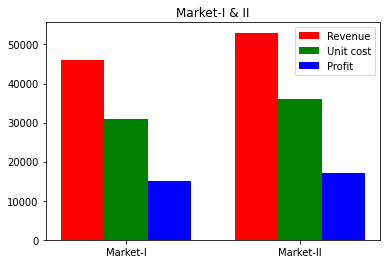
\includegraphics[width=\columnwidth]{solutions/su2021/45/FIGURE.png}
\caption{Revenue,Sales \& Profit Of Market-I \& II}
\label{matrix/2/45/fig:Profit}	
\end{figure}
  \item If A=$\myvec{\alpha &\beta\\ \gamma &-\alpha}$ is such that $A^{2}=I$,then\\
  (A)$1+\alpha^{2}+\beta\gamma=0$ (B)$1-\alpha^{}2+\beta\gamma=0$\\
  (C)$1-\alpha^{2}-\beta\gamma=0$ (D)$1+\alpha^{2}-\beta\gamma=0$\\
\\
\solution
%
\begin{align}
    E(X) &= \frac{1}{\sqrt{2\pi}} \int_{-\infty}^{\infty} x e^{-\frac{x^2}{2}}dx\\
    &=0 \quad \brak{ \text{ odd function}}
\end{align}
\begin{align}
    E\brak{X^2}&= \frac{1}{\sqrt{2\pi}}\int_{-\infty}^{\infty} x^2
e^ {-\frac{x^2}{2}} dx \quad \brak{even function}\\
    &= \frac{2}{\sqrt{2\pi}} \int_{0}^{\infty} x^2 e^{-\frac{x^2}{2}} dx\\
    &= \frac{2}{\sqrt{2\pi}}\int_{0}^{\infty}\sqrt{2u}e^{-u} du \quad\brak{Let \frac{x^2}{2}= u}\\
    &= \frac{2}{\sqrt{\pi}} \int_{0}^{\infty} e^{-u} u^{\frac{3}{2}-1} du\\
    &= \frac{2}{\sqrt{\pi}} \Gamma\brak{{\frac{3}{2}}}\\
    &= \frac{1}{\sqrt{\pi}}\Gamma\brak{\frac{1}{2}} \\
    &= 1
\end{align}
where we have used the fact that
\begin{align}
\quad\because \Gamma(n)= (n-1)\Gamma(n-1); \Gamma\brak{\frac{1}{2}}=\sqrt{\pi}
\end{align}
%
Thus, the  variance is
\begin{align}
    \sigma^2 =  E\brak X^2 - E^2\brak X = 1
\end{align}

  \item If the matrix A is both symmetric and skew symmetric,then\\
  (A) A is a diagonal matrix \\
  (B) A is a zero matriz\\
  (C)A is a square matrix \\
  (D)None of these\\
  \\
\solution
If $\vec{A}$ is symmetric, then 
\begin{align}
\vec{A}^T =\vec{A}
\label{matrix/48/2.0.1}
\end{align}
If matrix A is skew symmetric, then
\begin{align}
\vec{A}^T = \vec{-A}
\label{matrix/48/2.0.2}
\end{align}
From  \eqref{matrix/48/2.0.1} and \eqref{matrix/48/2.0.2},
\begin{align}
\vec{A} &=\vec{-A}
\\
\implies 2\vec{A} &= 0
\\
\text{or, } \vec{A} &= 0
\end{align}
$\therefore $ $\vec{A}$ is zero matrix.


  \item If A is square matrix such that $A^{2}=A$,then $(I+A)^{3}-7A$ is equal to\\
  (A)A \\(B)I-A\\ (C)I\\ (D)3A
\\
\solution
%
\begin{align}
    E(X) &= \frac{1}{\sqrt{2\pi}} \int_{-\infty}^{\infty} x e^{-\frac{x^2}{2}}dx\\
    &=0 \quad \brak{ \text{ odd function}}
\end{align}
\begin{align}
    E\brak{X^2}&= \frac{1}{\sqrt{2\pi}}\int_{-\infty}^{\infty} x^2
e^ {-\frac{x^2}{2}} dx \quad \brak{even function}\\
    &= \frac{2}{\sqrt{2\pi}} \int_{0}^{\infty} x^2 e^{-\frac{x^2}{2}} dx\\
    &= \frac{2}{\sqrt{2\pi}}\int_{0}^{\infty}\sqrt{2u}e^{-u} du \quad\brak{Let \frac{x^2}{2}= u}\\
    &= \frac{2}{\sqrt{\pi}} \int_{0}^{\infty} e^{-u} u^{\frac{3}{2}-1} du\\
    &= \frac{2}{\sqrt{\pi}} \Gamma\brak{{\frac{3}{2}}}\\
    &= \frac{1}{\sqrt{\pi}}\Gamma\brak{\frac{1}{2}} \\
    &= 1
\end{align}
where we have used the fact that
\begin{align}
\quad\because \Gamma(n)= (n-1)\Gamma(n-1); \Gamma\brak{\frac{1}{2}}=\sqrt{\pi}
\end{align}
%
Thus, the  variance is
\begin{align}
    \sigma^2 =  E\brak X^2 - E^2\brak X = 1
\end{align}

\item Balance the following chemical equation.
\begin{align}
  \label{matrix/50/eq1}
NaOH + H_2SO_4 \xrightarrow{} Na_2SO_4  +  H_2O
\end{align}
\\
\solution
Let the balanced version of \eqref{matrix/50/eq1} be
\begin{align}
   x_{1}NaOH + x_{2}H_2SO_4 \xrightarrow{} 
   x_{3}Na_2SO_4 + x_{4}H_2O \label{matrix/50/eq2}
\end{align}
which results in the following equations:
\begin{align}
    (x_{1}-2x_{3}) Na= 0\\
    (x_{1}+4x_{2}-4x_{3}-x_{4}) O= 0\\
    (x_{1}+2x_{2}-2x_{4}) H=0\\
    (x_{2}-x_{3}) S= 0
\end{align}
which can be expressed as
\begin{align}
    x_{1}+ 0.x_{2}- 2x_{3}+ 0.x_{4} = 0\\
    x_{1}+ 4x_{2}- 4x_{3}- x_{4} = 0\\
    x_{1}+ 2x_{2}+ 0.x_{3}- 2x_{4} = 0\\
    0.x_{1}+ x_{2}- x_{3}+ 0.x_{4} = 0
\end{align}
resulting in the matrix equation
\begin{align}
    \myvec{1 & 0 & -2 & 0\\
           1 & 4 & -4 & -1\\
           1 & 2 & 0 & -2\\
           0 & 1 & -1 & 0}\vec{x}
           =\vec{0}    \label{matrix/50/eq3}
\end{align}
where,
\begin{align}
   \vec{x}= \myvec{x_{1}\\x_{2}\\x_{3}\\x_{4}}
\end{align}
\eqref{matrix/50/eq3} can be reduced as follows:
\begin{align}
    \myvec{1 & 0 & -2 & 0\\
           1 & 4 & -4 & -1\\
           1 & 2 & 0 & -2\\
           0 & 1 & -1 & 0}
    \xleftrightarrow[R_{3}\leftarrow R_3-R_{1}]{R_{2}\leftarrow R_2- R_1}
    \myvec{1 & 0 & -2 & 0\\
           0 & 4 & -2 & -1\\
           0 & 2 & 2 & -2\\
           0 & 1 & -1 & 0}\\
    \xleftrightarrow{R_2 \leftarrow \frac{R_2}{4}}
    \myvec{1 & 0 & -2 & 0\\
          0 & 1 & -\frac{1}{2} & -\frac{1}{4}\\
          0 & 2 & 2 & -2\\
          0 & 1 & -1 & 0}\\
    \xleftrightarrow[R_4 \leftarrow R_4 - R_2]{R_3 \leftarrow R_3 - 2R_2}
    \myvec{1 & 0 & -2 & 0\\
           0 & 1 & -\frac{1}{2} & -\frac{1}{4}\\
           0 & 0 & 3 & -\frac{3}{2}\\
           0 & 0 & -\frac{1}{2} & \frac{1}{4}}\\
    \xleftrightarrow{R_3 \leftarrow \frac{R_3}{3}}
    \myvec{1 & 0 & -2 & 0\\
           0 & 1 & -\frac{1}{2} & -\frac{1}{4}\\
           0 & 0 & 1 & -\frac{1}{2}\\
           0 & 0 & -\frac{1}{2} & \frac{1}{4}}\\
    \xleftrightarrow[R_{4}\leftarrow R_4+\frac{R_3}{2}]{R_{2}\leftarrow R_2+ \frac{R_3}{2}}
    \myvec{1 & 0 & -2 & 0\\
           0 & 1 & 0 & -\frac{1}{2}\\
           0 & 0 & 1 & -\frac{1}{2}\\
           0 & 0 & 0 & 0}\\
    \xleftrightarrow{R_1 \leftarrow R_1+2R_3}
    \myvec{1 & 0 & 0 & -1\\
           0 & 1 & 0 & -\frac{1}{2}\\
           0 & 0 & 1 & -\frac{1}{2}\\
           0 & 0 & 0 & 0}
\end{align}
Thus,
\begin{align}
    x_1=x_4, x_2= \frac{1}{2}x_4, x_3=\frac{1}{2}x_4\\
    \implies \quad\vec{x}= x_4\myvec{1\\ \frac{1}{2}\\ \frac{1}{2}\\1} 
\end{align} 
by substituting $x_4= 2$
\begin{align}
    \vec{x}=\myvec{2\\1\\1\\2}
\end{align}
Hence, \eqref{matrix/50/eq2} finally becomes
\hfill\break
%\vspace{5mm}  finally becomes
\begin{align}
    2 NaOH + H_2SO_4 \xrightarrow{} 
    Na_2SO_4 + 2 H_2O
\end{align}
\item     Two farmers Ramkishan and Gurcharan Singh cultivate only three varieties of rice namely Basmati, Permal and Naura. The sale (in Rupees) of these varieties of rice by both the farmers in the month of September and October are given by the following matrices $\vec{A}$ and $\vec{B}$ .

\begin{center}
September Sales(in Rupees)
\end{center}
\begin{align}
    \vec{A}=
    \begin{blockarray}{cccc}
    \text{Basmati} & \text{Permal} & \text{Naura} \\
    \begin{block}{(ccc)(c)}
    10000 & 20000 & 30000 & \text{Ramkishan}\\
    50000 & 30000 & 10000 & \text{Gurucharan} \\
    \end{block}
    \end{blockarray}
\end{align}

\begin{center}
October Sales(in Rupees)
\end{center}
\begin{align}
    \vec{B} =
    \begin{blockarray}{cccc}
    \text{Basmati} & \text{Permal} & \text{Naura} \\
    \begin{block}{(ccc)(c)}
    5000 & 10000 & 6000 & \text{Ramkishan}\\
    20000 & 10000 & 10000 & \text{Gurucharan} \\
    \end{block}
    \end{blockarray}
\end{align}

\begin{enumerate}
    \item Find the combined sales in September and October for each farmer in each variety.
    \item Find the decrease in sales from September to October.
    \item If both farmers receive 2\% profit on gross sales, compute the profit for each farmer and for each variety sold in October.
\end{enumerate}
%
\solution

The given system of inequality can be written in matrix form as
\begin{align}
    \myvec{-1 & -2  \\ -1 & 1 \\ 1 & 1\\ 1 & 0 \\ 0 & 1}\vec{x} \succeq \myvec{-10\\0\\1\\0\\0}
\end{align}
which can be further simplified into 
\begin{align}
    \myvec{-1 & -2 \\ 1 & 0 \\ 0&1}\vec{x} \succeq \myvec{-10\\\frac{-1}{2}\\\frac{-1}{2}}
\end{align}
Let the surplus vector be
\begin{align}
    \vec{u} &= \myvec{u_1\\u_2} \succeq 0
\end{align}
\begin{enumerate}
    \item 
    \begin{align}
        \myvec{-1 & -2 \\ 1 & 0}\vec{x} &\succeq \myvec{-10 \\ \frac{-1}{2}}
        \\
        \implies  \myvec{-1 & -2 \\ 1 & 0}\vec{x} &= \myvec{-10 \\ \frac{-1}{2}} + \vec{u}
    \end{align}
    resulting in 
    \begin{align}
        \vec{x} &= \myvec{-1 & -2 \\ 1 & 0}^{-1}\myvec{-10 \\\frac{-1}{2}} + \myvec{-1 & -2 \\ 1 & 0}^{-1}\vec{u}
        \\
        \implies \vec{x} &= \myvec{\frac{1}{2} \\ \frac{19}{4}} + \myvec{0&1\\ \frac{-1}{2}&\frac{-1}{2}}\vec{u}   \label{ineq/58/eq1}
    \end{align}
    \item 
    \begin{align}
        \myvec{-1& -2 \\ 0 & 1}\vec{x} &\succeq \myvec{-10 \\ \frac{-1}{2}}
        \\
        \implies  \myvec{-1& -2 \\ 0 & 1}\vec{x} &= \myvec{-10 \\ \frac{-1}{2}} + \vec{u}
    \end{align}
    resulting in 
    \begin{align}
        \vec{x} &= \myvec{-1& -2 \\ 0 & 1}^{-1}\myvec{-10 \\ \frac{-1}{2}} + \myvec{-1& -2 \\ 0 & 1}^{-1}\vec{u}
        \\
        \implies \vec{x} &= \myvec{9\\\frac{1}{2}} + \myvec{-1& -2 \\ 0 & 1}\vec{u} \label{ineq/58/eq2}
    \end{align}
\end{enumerate}
Now,solution region which is common to regions of eq. \eqref{ineq/58/eq1} and eq. \eqref{ineq/58/eq2},is given by
\begin{align}
    \boxed{\vec{x} = \myvec{\frac{1}{2}\\\frac{1}{2}}+\myvec{0&1\\\frac{-1}{2}&1}\vec{u}}
\end{align}
%
\begin{figure}[!ht]
\centering
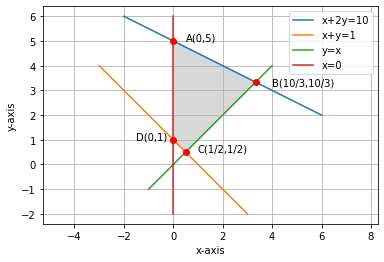
\includegraphics[width=\columnwidth]{solutions/su2021/2/58/Figures/Figure_2.58.png}
\caption{Graphical Solution}
\label{ineq/58/fig:fig1}	
\end{figure}

\begin{figure}[!ht]
\centering
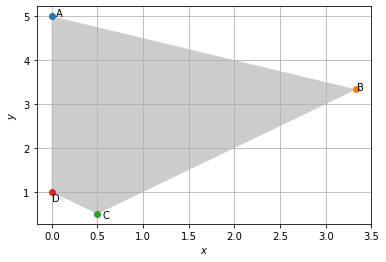
\includegraphics[width=\columnwidth]{solutions/su2021/2/58/Figures/2.58(2).png}
\caption{Magnified Solution region}
\label{ineq/58/fig:fig2}	
\end{figure}


\item If A=$\myvec{1 &2 &3\\3 &-2 &1\\4 &2 &1}$,then show that $A^3-23A-40I=0$
\\  
\solution
Given that $\vec{A}$ =$\myvec{1&2&3\\3&-2&1\\4&2&1}$.
\begin{enumerate}
\item \textbf{The Characteristic equation} is given by:
\begin{align}
  \implies  \abs{\vec{A}-\lambda\vec{I}}&=0
    \\
    \implies \mydet{1-\lambda&2&3\\3&-2-\lambda&1\\4&2&1-\lambda}&=0
    \end{align}
\begin{multline}
   \implies\brak{1-\lambda}\brak{\brak{-2-\lambda}\brak{1-\lambda}-2}
   \\
   -2\brak{3\brak{1-\lambda}-4}+3\brak{6+4\brak{2+\lambda}}=0
\end{multline}
\begin{align}
 \implies   \lambda^3-23\lambda-40=0
\end{align}
The above equation is similar to equation to be proved.
\item According to \textbf{Cayley-Hamilton Theorem:} 
\\
Every square matrix satisfies its own
\\\textbf{characteristic equation}.
\begin{align}
\therefore    \vec{A}^3-23\vec{A}-40\vec{I}=0
\end{align}
Hence Proved.
\end{enumerate}
\item In a legislative assembly election, a political
group hired a public relations firm to promote
its candidate in three ways: telephone, house
calls, and letters. The cost per contact (in paise)
is given in matrix $\vec{A}$ as
\begin{center}
Cost per Contact(in Paise)
\end{center}
\begin{align}
    \vec{A}=
    \begin{blockarray}{cc}
    \text{cost}\\
    \begin{block}{(c)(c)}
    40 &\text{Telephone}\\
    100&\text{Housecall} \\
    50&\text{Letter}\\
    \end{block}
    \end{blockarray}
\end{align}
The number of contacts of each type made in
two cities X and Y is given by matrix $\vec{B}$
\begin{align}
    \vec{B} =
    \begin{blockarray}{cccc}
    \text{Telephone} & \text{Housecall} & \text{Letter} \\
    \begin{block}{(ccc)(c)}
    1000 & 500 & 5000 & \text{X}\\
    3000 & 1000 & 10000 & \text{Y} \\
    \end{block}
    \end{blockarray}
\end{align}
Find the total
amount spent by the group in the two cities
X and Y
%
\solution

The total amount spent is given by=

    \begin{multline}
    \vec{B}\vec{A}\\
    =\myvec{1000&500&5000\\3000&1000&10000}\myvec{40\\100\\50}\\
    =\myvec{40000+50000+250000\\120000+100000+500000}\\
    \begin{blockarray}{cc}
    \text{TotalCost} \\
    \begin{block}{(c)(c)}
    340000&\text{X}\\
    720000&\text{Y}\\
    \end{block}
    \end{blockarray}
    \end{multline}
$\therefore$ the total amount spent in city X and city Y is 3400 and 7200 Rupees respectively.  See Fig. \ref{matrix/64fig:Profit}	
%
\begin{figure}[!ht]
\centering
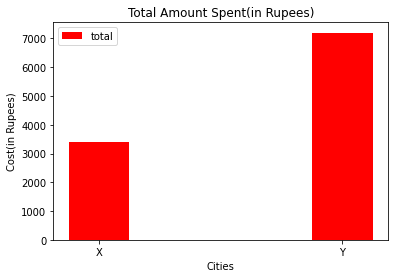
\includegraphics[width=\columnwidth]{solutions/su2021/64/figure8.png}
\caption{Total Amount Spent by the group in cities X and Y}
\label{matrix/64fig:Profit}	
\end{figure}

\item Express the matrix B=$\myvec{2 &-2 &-4\\-1 &3 &4\\1 &-2 &-3}$ as the sum of a symmetric and a skew symmetric matrix.\\
\solution
  We obtain the vertices of the rhombus as follows
\begin{align}
\vec{A} = \myvec{-3\\0},
\vec{B} = \myvec{0\\-3.5},
\vec{C} = \myvec{3\\0},
\vec{D} = \myvec{0\\3.5}
\end{align}
which are plotted in Fig. \ref{quad/45/fig:Rhombus ABCD}.
%
\begin{figure}[ht!]
\centering
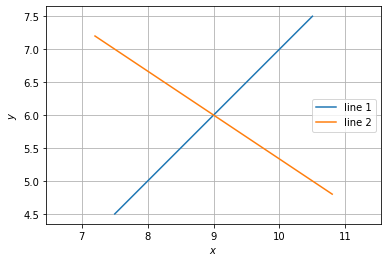
\includegraphics[width=\columnwidth]{solutions/quad/45/figure2.png}
\caption{Rhombus ABCD}
\label{quad/45/fig:Rhombus ABCD}
\end{figure}

  \item Obtain the inverse of the following matrix using elementary operations\\
  A=$\myvec{0 &1 &2\\1 &2 &3\\3 &1 &1}$.\\
  \solution
    \begin{enumerate}
    \item Given that
    \begin{align}
    \vec{A}& =\myvec {0 & 1 & 2\\1 & 2 & 3\\3 & 1 & 1}
    \end{align}
     The augmented matrix $[A | I]$ is as given below:- 
    \begin{align}
    \myvec{0 & 1 & 2 & \vrule & 1 & 0 & 0\\1 & 2 & 3 & \vrule & 0 & 1 & 0\\3 & 1 & 1 & \vrule & 0 & 0 & 1}
    \end{align}
    We apply the elementary row operations on $[A | I]$ as follows :-
    \begin{align}
    [A | I] = \myvec{0 & 1 & 2 & \vrule & 1 & 0 & 0\\1 & 2 & 3 & \vrule & 0 & 1 & 0\\3 & 1 & 1 & \vrule & 0 & 0 & 1}
    \\
    \xleftrightarrow{R_1\leftrightarrow R_2}   
    \myvec{1 & 2 & 3 & \vrule & 0 & 1 & 0\\0 & 1 & 2 & \vrule & 1 & 0 & 0\\3 & 1 & 1 & \vrule & 0 & 0 & 1}
    \\
    \xleftrightarrow{R_3\leftarrow R_3-3R_1}   
    \myvec{1 & 2 & 3 & \vrule & 0 & 1 & 0\\0 & 1 & 2 & \vrule & 1 & 0 & 0\\0 & -5 & -8 & \vrule & 0 & -3 & 1}
    \\
    \xleftrightarrow{R_1\leftarrow R_1-2R_2}  
    \myvec{1 & 0 & -1 & \vrule & -2 & 1 & 0\\0 & 1 & 2 & \vrule & 1 & 0 & 0\\0 & -5 & -8 & \vrule & 0 & -3 & 1}
    \\
    \xleftrightarrow{R_3\leftarrow R_3+5R_2}  
    \myvec{1 & 0 & -1 & \vrule & -2 & 1 & 0\\0 & 1 & 2 & \vrule & 1 & 0 & 0\\0 & 0 & 2 & \vrule & 5 & -3 & 1}
    \\
    \xleftrightarrow{R_3\leftarrow R_3/2}
    \myvec{1 & 0 & -1 & \vrule & -2 & 1 & 0\\ 0 & 1 & 2 & \vrule & 1 & 0 & 0\\0 & 0 & 1 &\vrule &\frac{5}{2} &\frac{-3}{2} &\frac{1}{2}}
    \\
    \xleftrightarrow{R_1\leftarrow R_1+R_3}
    \myvec{1 & 0 & 0 & \vrule & \frac{1}{2} & \frac{-1}{2} & \frac{1}{2}\\ 0 & 1 & 2 & \vrule & 1 & 0 & 0\\0 & 0 & 1 &\vrule &\frac{5}{2} &\frac{-3}{2} &\frac{1}{2}}
    \\
    \xleftrightarrow{R_2\leftarrow R_2-2R_3}
    \myvec{1 & 0 & 0 & \vrule & \frac{1}{2} & \frac{-1}{2} & \frac{1}{2}\\ 0 & 1 & 0 & \vrule & -4 & 3 & -1\\0 & 0 & 1 &\vrule &\frac{5}{2} &\frac{-3}{2} &\frac{1}{2}}
    \end{align}
    By performing elementary transformations on augmented matrix$ [A | I]$ , we obtained the augmented matrix in the form $ [I | A]$. 
    Hence we can conclude that the matrix A is invertible and inverse of the matrix is:-
    \begin{align}
    \therefore\vec{A^{-1}}=\myvec { \frac{1}{2} & \frac{-1}{2} & \frac{1}{2} \\  -4 & 3 & -1\\ \frac{5}{2} &\frac{-3}{2} &\frac{1}{2}}
    \end{align}
    \item QR decomposition of  \myvec{0  & 1 & 3 \\ 1 & 2 & 3 \\ 2 & 3 & 1}
    \\
     Let us use the Gram-schmidt approach to obtain QR decomposition of$ \vec{A}$. Consider rows vectors say $\vec{a_1}$,$\vec{a_2}$ and $\vec{a_3}$ of $\vec{A}$  which is given by
    \begin{align}
    \vec{a_1}=\myvec{0 & 1 & 2}\label{matrix/69/eq1}\\
    \vec{a_2}=\myvec{1 & 2 & 3}\label{matrix/69/eq2}\\
    \vec{a_3}=\myvec{3 & 1 & 1}\label{matrix/69/eq3}
    \end{align}
    we can express these as 
    \begin{align}
    \vec{u_1}&=\vec{a_1}=\myvec{0 & 1 & 2}\label{matrix/69/eq4}\\
    \vec{e_1}&=\frac{\vec{u_1}}{\norm{\vec{u_1}}}\\
    \vec{e_1}&=\frac{\myvec{0 & 1 & 2}}{\sqrt{0+1+4}}\\
    \vec{e_1}&=\myvec{0 & \frac{1}{\sqrt{5}} & \frac{2}{\sqrt{5}}}\\
    \vec{u_2}&=\vec{a_2}-(\vec{a_2}\vec{e_1})\vec{e_1}\\
    &=\myvec{1 & 2 & 3}-(\myvec{1 & 2 & 3}\myvec{0 & \frac{1}{\sqrt{5}} & \frac{2}{\sqrt{5}}})\myvec{0 & \frac{1}{\sqrt{5}} &  \frac{2}{\sqrt{5}}}\\
    &=\myvec{1 & \frac{2}{5} & \frac{-1}{5}}\\
    \vec{e_2}&=\frac{\vec{u_2}}{\norm{\vec{u_2}}}=\frac{\myvec{1 & \frac{2}{5} & \frac{-1}{5}}}{\sqrt{1+\frac{4}{25}+\frac{1}{25}}}\\
    \vec{e_2}&=\myvec{\frac{5}{\sqrt{30}} & \frac{2}{\sqrt{30}} &\frac{-1}{\sqrt{30}}}\\
    \vec{u_3}&=\vec{a_3}-(\vec{a_3}\vec{e_1})\vec{e_1}-(\vec{a_3}\vec{e_2})\vec{e_2}
    \\
    \vec{u_3}&=\myvec{\frac{1}{3} & \frac{-2}{3} &\frac{1}{3}}\\
    \vec{e_3}&=\frac{\vec{u_3}}{\norm{\vec{u_3}}}\\
    &=\frac{\myvec{\frac{1}{3} & \frac{-2}{3} & \frac{1}{4}}}{\sqrt{\frac{1}{9}+\frac{4}{9}+\frac{1}{9}}}\\
    \vec{e_3}&=\myvec{\frac{1}{\sqrt{6}} & \frac{-2}{\sqrt{6}} &\frac{1}{\sqrt{6}}}
    \end{align}
    Thus,
    \begin{align}
     \vec{Q}&=(e_1|e_2|----|e_n)\\
     &=\myvec{0 & \frac{5}{\sqrt{30}} & \frac{1}{\sqrt{6}}\\\frac{1}{\sqrt{5}} & \frac{2}{\sqrt{30}} & \frac{-2}{\sqrt{6}}\\\frac{2}{\sqrt{5}} & \frac{-1}{\sqrt{30}} & \frac{1}{\sqrt{6}}}\label{matrix/69/eq5}      
    \end{align}
    Then
    \begin{align}
      \vec{R}&=\myvec{a_1e_1 & a_2e_1 & a_3e_1\\ 0 & a_2e_2 & a_3e_2\\0 & 0 & a_3e_3}\\
      &=\myvec{\frac{5}{\sqrt{5}} & \frac{8}{\sqrt{5}} & \frac{3}{\sqrt{5}}\\0 &  \frac{6}{\sqrt{30}} & \frac{16}{\sqrt{30}}\\0 & 0 & \frac{2}{\sqrt{6}}}\label{matrix/69/eq6} 
      \end{align}
    From equations \eqref{matrix/69/eq5} and \eqref{matrix/69/eq6} the obtained $\vec{Q} \vec{R}$ Decomposition is
    \begin{align}
     \myvec{0  & 1 & 3 \\ 1 & 2 & 3 \\ 2 & 3 & 1}&= \myvec{0 & \frac{5}{\sqrt{30}} & \frac{1}{\sqrt{6}}\\\frac{1}{\sqrt{5}} & \frac{2}{\sqrt{30}} & \frac{-2}{\sqrt{6}}\\\frac{2}{\sqrt{5}} & \frac{-1}{\sqrt{30}} & \frac{1}{\sqrt{6}}}\myvec{\frac{5}{\sqrt{5}} & \frac{8}{\sqrt{5}} & \frac{3}{\sqrt{5}}\\0 &  \frac{6}{\sqrt{30}} & \frac{16}{\sqrt{30}}\\0 & 0 & \frac{2}{\sqrt{6}}} 
    \end{align}
    \end{enumerate}
    \item Find P$^{-1}$, if it exists, given \\
    P=$\myvec{10 &-2\\-5 &1}$.\\
    \solution
    Using row reduction, 
%
\begin{align}
\myvec{10 & -2 \\-5 & 1}
\xleftrightarrow {R_2 \leftarrow R_2+\frac{R_1}{2}}\myvec{10& -2& \\0 & 0}
\end{align} 
Hence,  $\vec {P}^{-1} $ does not exist.
     
%\end{enumerate}
%\end{document}
    
